%====================================================================================================
% ?????
%====================================================================================================
% TCC
%----------------------------------------------------------------------------------------------------
% Autor				: Jasane Schio
% Orientador		: Gedson Faria
% Co-Orientador		: Angelo Darcy
% Instituição 		: UFMS - Universidade Federal do Mato Grosso do Sul
% Departamento		: CPCX - Sistema de Informação
%----------------------------------------------------------------------------------------------------
% Data de criação	: 01 de Outubro de 2015
%====================================================================================================
% NO FUTURO
\chapter{Resultados} 

Para obtenção dos resultados foram organizados dois tipos de testes: Teste por região e
Teste geral.

No teste por região o campo foi dividido verticalmente em cinco faixas e cada faixa dividia em três partes horizontais. Cada uma das faixas possue ao seu centro um conjunto de cinco cores.
Cada faixa horizontal possui vinte e nove centimetros, já as faixas verticais possuem quarenta e um centimetros com um intervalo de um centimetro entre elas.

Em cada ponto de teste estão disposta cinco cores: Vermelho  e Verde na primeira linha, Amarelo, Azul e Laranja na segunda. As cores estão distantes verticalmente \textit{7.5cm}, na primeria linha a distancia entre as cores é  de \textit{11 cm} e na segunda linha de \textit{7.2 cm}. Um  melhor detalhamento da disposiçao das cores é  mostrado na Figura \ref{disposicaoparte}.

\begin{figure}[!: h]
		\centering
		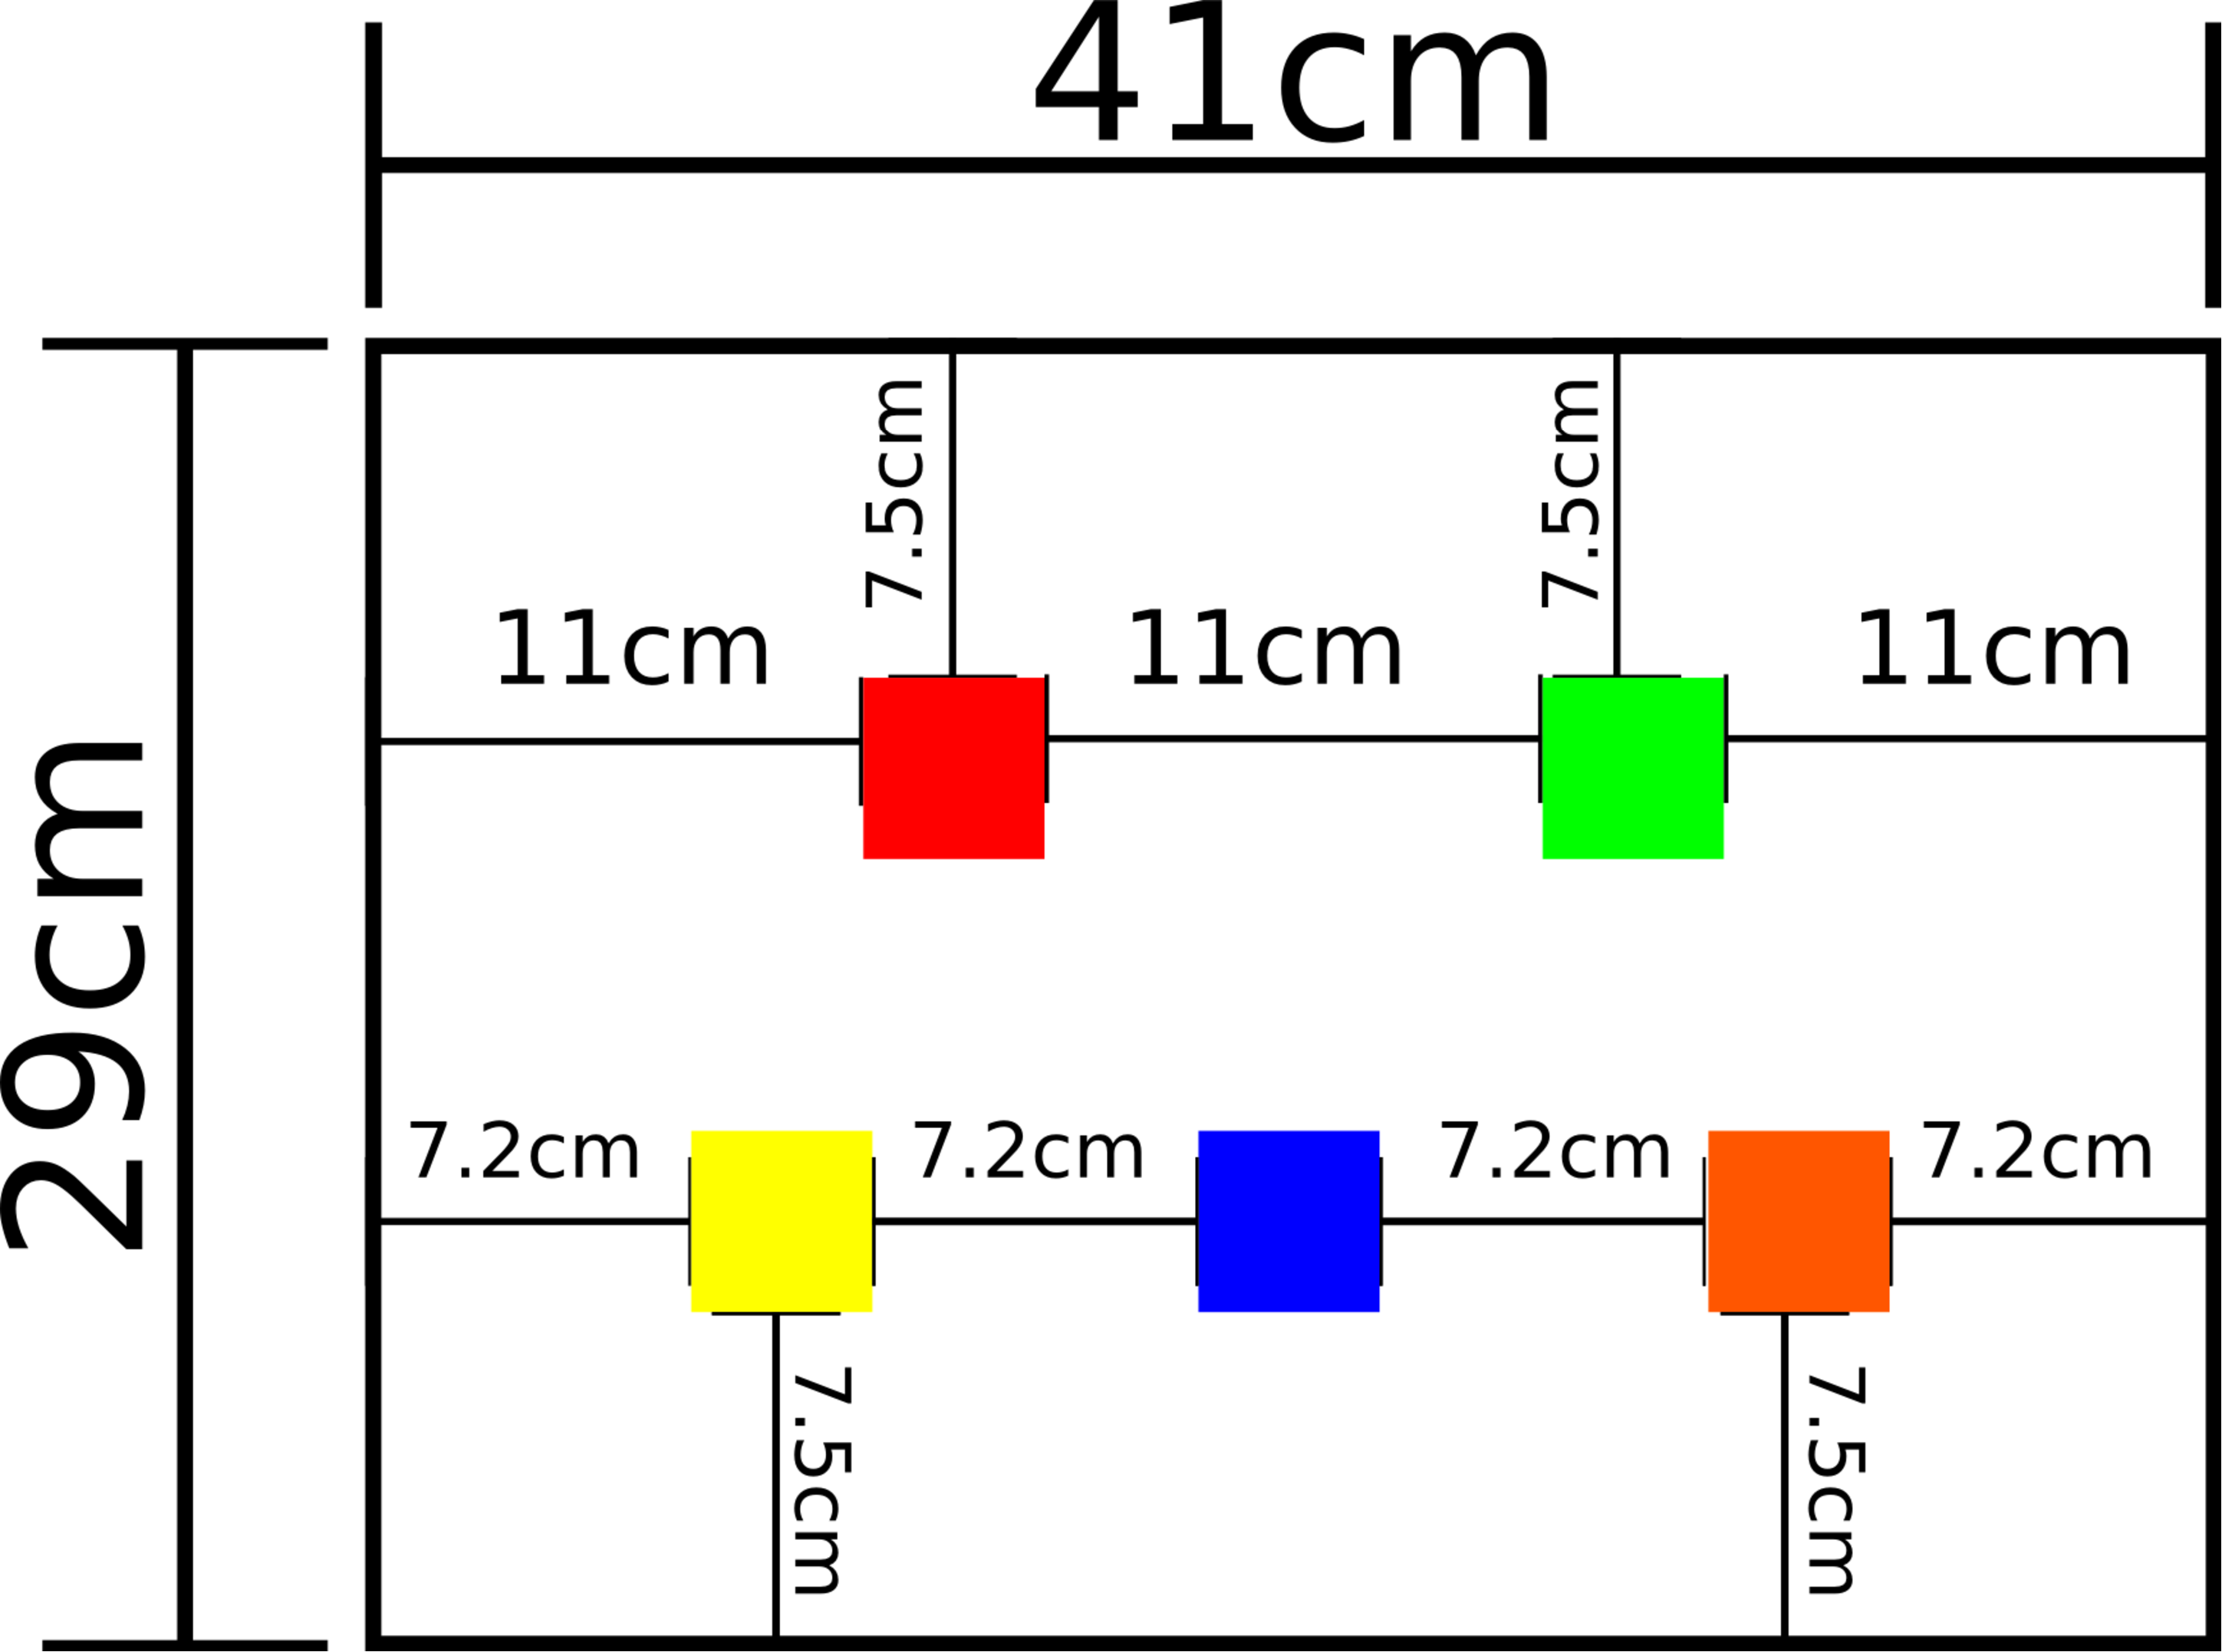
\includegraphics[width=0.4\textwidth]{disposicaoparte.pdf}
		\caption{Disposição dos objetos coloridos dentro de cada uma das partes}
		\label{disposicaoparte}
	\end{figure}
	
No total estavam disposto no campo quinze pontos de cada cor, sendo as cores: . Sendo cinco areas horizontais e três verticais, a divisão do campo resulta em quinze partes, cada um das partes sera testada vinte e cinco vezes.
 Para cada uma das faixas foram testadas calibrações com cinco tipos diferentes de contraste e luminosidade, somando um total de vinte e cinco testes.	
	
	
\begin{table}[h]
\centering
\caption{Tabela de Testes}
\begin{tabular}{r|lr}
Tipo de Teste & Quantidade \\ % Note a separação de col. e a quebra de linhas
\hline                               % para uma linha horizontal
Divisões no Campo        & 25 \\
Constrate  & 5\\
Brilho            & 5 \\
\hline  
Total & 260
 
\end{tabular}
\end{table}
